\begin{frame}
	\frametitle{Transazioni $\rightarrow$ Blocchi} 
	\framesubtitle{generazione nuova transazione}
	
	\begin{enumerate}
		\item broadcastata tramite protocollo \textit{flooding}
		\item ogni miner \textbf{può} includerla nel suo \textit{pool}
		\item inizialmente inserita in un pool come \textit{invalida}
		\item dopo risoluzione del $\mathfrak{B}$ corrente è rimossa da ogni pool
	\end{enumerate}

	\begin{figure}[H]
		\begin{center}
			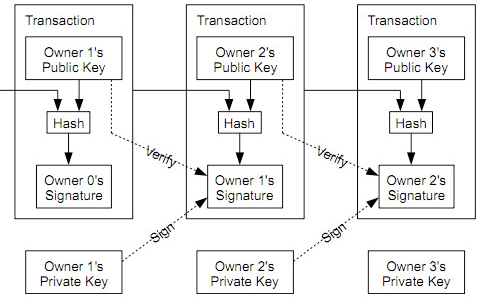
\includegraphics[height = 4.5 cm]{images/chain_transactions.png}	
		\end{center}
	\end{figure}
\end{frame}